\documentclass[aspectratio=1610,table]{beamer}
\usepackage[british]{babel}
\usepackage[utf8]{inputenc}
\usepackage{amsmath,amsfonts,amssymb}
\usepackage{relsize}
\usepackage{xfrac,unicode-math}
\usepackage{hyperref}
\usepackage{textpos}
\usepackage{graphicx}
\usepackage{multicol}
\usepackage{hyperref}
\usepackage{tikz}
\usepackage{stmaryrd}

\defaultfontfeatures{Scale=MatchLowercase}
\usepackage{pdfcomment}
\newcommand{\pdfnote}[1]{\marginnote{\pdfcomment[icon=note]{#1}}}

\def\<#1>{{\textsmaller{#1}}}

\usetheme{Madrid}
\usecolortheme{beaver}
\definecolor{darkred}{rgb}{0.8,0,0}
\definecolor{darkgreen}{rgb}{0,0.8,0}
\setbeamercolor{structure}{fg=darkred}
\usetikzlibrary{shapes.geometric,calc,arrows}
\newcommand\score[2]{
\pgfmathsetmacro\pgfxa{#1+1}
\tikzstyle{scorestars}=[star, star points=5, star point ratio=2.25, draw,inner sep=1.3pt,anchor=outer point 3]
  \begin{tikzpicture}[baseline]
    \foreach \i in {1,...,#2} {
    \pgfmathparse{(\i<=#2-#1?"white":"black")}
    \edef\starcolor{\pgfmathresult}
    \draw (\i*1.75ex,0) node[name=star\i,scorestars,fill=\starcolor]  {};
   }
  \end{tikzpicture}
}
\DeclareMathOperator*{\argmax}{arg\,max} % thin space, limits underneath in displays
\DeclareMathOperator*{\rnd}{rnd}


\beamertemplatenavigationsymbolsempty

\makeatletter
\setbeamertemplate{footline}
{
  \leavevmode%
  \hbox{%
  \begin{beamercolorbox}[wd=.333333\paperwidth,ht=4.8ex,dp=1ex,center]{author in head/foot}%
    \usebeamerfont{author in head/foot}\inserttitle
  \end{beamercolorbox}%
  \begin{beamercolorbox}[wd=.333333\paperwidth,ht=2.96ex,dp=1ex,center]{title in head/foot}%
    \usebeamerfont{title in head/foot}Kevin Dreßler
  \end{beamercolorbox}%
  \begin{beamercolorbox}[wd=.333333\paperwidth,ht=2.96ex,dp=1ex,right]{date in head/foot}%
    \usebeamerfont{date in head/foot}%\insertshortdate{}\hspace*{5em}
    \insertframenumber{} / \inserttotalframenumber\hspace*{2.5ex} 
  \end{beamercolorbox}}%
  \begin{textblock*}{100mm}(.89\textwidth,-12.5mm)
    \includegraphics[height=8mm,width=8mm]{gfx/uni_leipzig_logo.pdf}
    \includegraphics[height=8mm,width=8mm]{gfx/dice_logo_small.png}
  \end{textblock*}
  \vskip0pt%
}
\makeatother

\usepackage{float}
\newfloat{myfloat}{t}{lop}

\usepackage{listings}
\lstset{ %this is the stype
        mathescape=true,
        frame=tB,
        numbers=left, 
        numberstyle=\tiny,
        basicstyle=\scriptsize, 
        keywordstyle=\color{darkred}\bfseries\em,
        commentstyle=\color{darkred}\ttfamily,
        morecomment=[f][\color{red}]{\#},
        keywords={,input, output, return, datatype, function, in, if, else, foreach, while, begin, end, } %add the keywords you want, or load a language as Rubens explains in his comment above.
        numbers=left,
        xleftmargin=.04\textwidth,
    }
    
\addtobeamertemplate{frametitle}{
   \let\insertframetitle\insertsectionhead}{}
\addtobeamertemplate{frametitle}{
   \let\insertframesubtitle\insertframetitle}{}


\makeatletter
  \CheckCommand*\beamer@checkframetitle{\@ifnextchar\bgroup\beamer@inlineframetitle{}}
  \renewcommand*\beamer@checkframetitle{\global\let\beamer@frametitle\relax\@ifnextchar\bgroup\beamer@inlineframetitle{}}
\makeatother


% ****************************************************************************************************



%\setbeamertemplate{footline}[title;frame number]

%\setbeamercolor{block title}{fg=white,bg=blue!75!black}

\newcommand\blfootnote[1]{%
  \begingroup
  \renewcommand\thefootnote{}\footnote{#1}%
  \addtocounter{footnote}{-1}%
  \endgroup
}


\setbeamertemplate{subsection page}
{
  \begin{centering}   
  {\usebeamerfont{subsection name}\usebeamercolor[fg]{subsection name}\insertsection}
    \vskip1em\par
    \begin{beamercolorbox}[sep=4pt,center]{part title}
      \usebeamerfont{subsection title}\insertsubsection\par
    \end{beamercolorbox}
  \end{centering}
}
%\AtBeginSubsection{\frame{\subsectionpage}}
%\AtBeginSection{\frame{\sectionpage}}
\setmathfont{TeX Gyre Pagella Math}
\begin{document}

\title{Learning Arbitrary RDF Dataset Enrichment Graphs Using Pre-~\&~Postcondition Broadcasting}
\author{\includegraphics[height=2cm]{gfx/uni_leipzig_logo}\qquad\includegraphics[height=2cm]{gfx/dice_logo.png}\\\medskip \medskip Kevin Dreßler}
\institute{Institut für Informatik \\ Universität Leipzig \\ DICE The Data Science Group}
\date{19.07.2019}

{ \setbeamertemplate{footline}{} 
\frame{\titlepage}
}
\addtobeamertemplate{frametitle}{}{%
}
\addtocounter{framenumber}{-1}
\setbeamercovered{invisible}

{ \setbeamertemplate{footline}{} 
\begin{frame}<beamer>{Outline}
    \tableofcontents
\end{frame}
}
\addtocounter{framenumber}{-1}
%\beamerdefaultoverlayspecification{<+->}


%%% Content %%%

\section{Motivation}

\begin{frame}{Linked Data Integration}
\begin{multicols}{2}
{\begin{center}
\includegraphics[width=0.5\textwidth]{gfx/flow}\end{center}}
{~~\smallskip
\begin{itemize}[<+->]
  \item Publishing 5-Star Linked Open Data (LOD)
  \item Flexible distribution of datasets to customers
  \item Investigating research questions
  \item Preparing data for experiments
  \item Integrating LOD into business applications
\end{itemize}}
\end{multicols}
\end{frame}


\begin{frame}{Linked Data Integration Steps}
\begin{multicols}{2}
{\begin{center}
\includegraphics[width=0.5\textwidth]{gfx/flow}\end{center}}
{~~\smallskip
\begin{itemize}[<+->]
  \item Lifting
  \item Fusion
  \item Linking
  \item{ \textbf{Enrichment}\\$\,\to$RDF Dataset Enrichment Framework (\<DEER>)}
\end{itemize}}
\end{multicols}
\end{frame}


\begin{frame}{RDF Dataset Enrichment Framework (\<DEER>)}
\begin{textblock*}{5cm}(11.0cm, -0.5cm) % {block width} (coords)
\includegraphics[width=5cm]{gfx/deer}
\end{textblock*}
\begin{itemize}[<+->]
  \item Generalistic framework for RDF dataset enrichment
  \item Goal: accessible easy enrichment for non-experts  
  \item Enrichment represented as pipelines
  \item Most enrichment functions need configuration
  \item $\to$ Requires expert knowledge $\lightning$
  \item $\to$ Try to use machine learning
\end{itemize}
\end{frame}

%\subsection{Objective of the Thesis}
\begin{frame}{ML Algorithm in original \<DEER>}
\begin{textblock*}{5cm}(11.0cm, -0.5cm) % {block width} (coords)
\includegraphics[width=5cm]{gfx/deer}
\end{textblock*}
\begin{itemize}
  \item Training data: RDF Datasets Source ($S$) and Target ($T$)
  \item Fitness Function: $F_1$ score over triples
  \item Iterative construction with an upward refinement operator
  \item Good theoretical properties \small{(finite, proper, complete, not redundant)}
\end{itemize}
\end{frame}
\begin{frame}{Analysis of Existing ML Algorithm in \<DEER>}
\begin{itemize}[<+->]
  \item But several incorrect implicit assumptions
  \begin{itemize}
    \item Sequential chaining is sufficient for arbitrary enrichment $\lightning$
\pdfnote{problematic due to un-awareness of other enrichment functions (modularity) and information loss}
    \item $F_1$ score over triples is a good fitness measure $\lightning$
\pdfnote{Partial increase in fitness can not detected}
    \item Enrichment Operators are independent $\lightning$
\pdfnote{Counterexample: Linking $\to$ Dereferencing}
    \item Training data always contains sufficient information for deterministic self-configuration $\lightning$
\pdfnote{possible, but not realistic,at least as hard to satisfy as manual configuration}
  \end{itemize}
  \item $\to$ Objective of this thesis: develop new approach (\<DEER2>)
\end{itemize}
\end{frame}
\begin{frame}{Derived Goals \& Research Questions}
\begin{itemize}[<+->]
  \item Design goals: \<DEER2> should 
\begin{itemize}
  \item[\textbf{(G1)}] be highly modular
  \item[\textbf{(G2)}] represent RDF dataset enrichment workflows efficiently as \<DAG>
  \item[\textbf{(G3)}] include an optimized, \<GP> based learning algorithm
  \item[\textbf{(G4)}] improve on all of the identified shortcomings of \<DEER>.
\end{itemize}
\item Research questions w.r.t. learning algorithm:
\begin{itemize}
  \item[\textbf{(Q1)}] What is the optimal set of hyperparameters?
  \item[\textbf{(Q2)}] How does our approach perform on real world datasets?
\end{itemize}
\end{itemize}
\end{frame}
\section{Approach}
\subsection{Classification of Enrichment Graphs}

\begin{frame}{Definitions}
\begin{figure}[tb]
\centering
  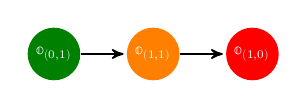
\begin{tikzpicture}[->,>=stealth',shorten >=1pt,auto,node distance=2.1cm,
                    semithick,scale=0.6, every node/.style={scale=0.6}]

  \node[shape=circle,fill=black!50!green,draw=none,text=white] (B)  {$\mathbb{o}_{(0,1)}$};
  \node[shape=circle,fill=orange,draw=none,text=white] (A) [right of=B]                   {$\mathbb{o}_{(1,1)}$};
  \node[shape=circle,fill=red,draw=none,text=white] (F) [right of=A]       {$\mathbb{o}_{(1,0)}$};


  \path (B) edge node [sloped, above] {} (A)
        (A) edge node [sloped, above] {} (F);
\end{tikzpicture}
\end{figure}\begin{block}{Definition \textbf{Dataset Operator}}
%Let $\mathcal{D}$ be the set of all RDF Datasets.
%A function
\begin{equation*}
\begin{aligned}
\mathbb{o}_{(n,m)}\colon \mathcal{D}^n \times  \mathcal{D}  &\to \mathcal{D}^m \\
\left(\left(D_{1}^{(\text{in})}, \dots, D_{n}^{(\text{in})}\right), P\right) & \mapsto \left( D_{1}^{(\text{out})}, \dots, D_{m}^{(\text{out})} \right)
\end{aligned}
\end{equation*}
%is called a \textbf{dataset operator}.\\
%We call $n$ the in-degree and $m$ the out-degree of $\mathbb{o}_{(n,m)}$.\\
%The set of all dataset operators is denoted as $\mathbb{O}$.
\begin{itemize}[<+->]
  \item $\mathbb{o}_{(0,1)}$ is called a \textbf{dataset emitter},
  \item $\mathbb{o}_{(1,0)}$ is called a \textbf{dataset acceptor},
  \item $\mathbb{o}_{(n,m)}$ is called an \textbf{enrichment operator} for $n,m>0$ and
  \item $\mathbb{o}_{(n,1)}$ is called a \textbf{confluent enrichment operator}.
\end{itemize}

\end{block}

\end{frame}

\begin{frame}{Definitions (Cont.)}

\begin{multicols}{3}
\begin{center}
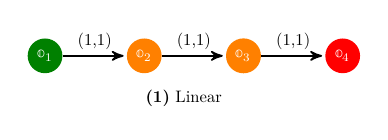
\begin{tikzpicture}[->,>=stealth',shorten >=1pt,auto,node distance=2.1cm,
                    semithick,scale=0.6, every node/.style={scale=0.6}]

  \node[shape=circle,fill=black!50!green,draw=none,text=white] (B)  {$\mathbb{o}_1$};
  \node[shape=circle,fill=orange,draw=none,text=white] (A) [right of=B]                   {$\mathbb{o}_2$};
  \node[shape=circle,fill=orange,draw=none,text=white] (E) [right of=A]       {$\mathbb{o}_3$};
  \node[shape=circle,fill=red,draw=none,text=white] (F) [right of=E]       {$\mathbb{o}_4$};
  \node[anchor=west] at (2,-0.9) (X) {\textbf{(1)} Linear};

  \path (A) edge node [sloped, above] {(1,1)} (E)
        (B) edge node [sloped, above] {(1,1)} (A)
        (E) edge node [sloped, above] {(1,1)} (F);
\end{tikzpicture}
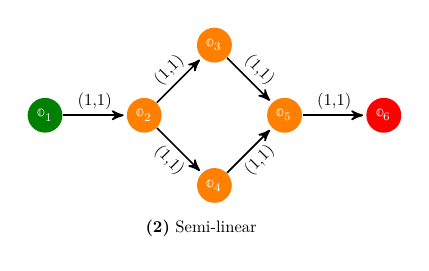
\begin{tikzpicture}[->,>=stealth',shorten >=1pt,auto,node distance=2.1cm,
                    semithick,scale=0.6, every node/.style={scale=0.6}]

  \node[shape=circle,fill=black!50!green,draw=none,text=white] (B)  {$\mathbb{o}_1$};
  \node[shape=circle,fill=orange,draw=none,text=white] (A) [right of=B]                   {$\mathbb{o}_2$};
  \node[shape=circle,fill=orange,draw=none,text=white] (C) [above right of=A]   {$\mathbb{o}_3$};
  \node[shape=circle,fill=orange,draw=none,text=white] (D) [below right of=A]  {$\mathbb{o}_4$};
  \node[shape=circle,fill=orange,draw=none,text=white] (E) [above right of=D]       {$\mathbb{o}_5$};
  \node[shape=circle,fill=red,draw=none,text=white] (F) [right of=E]       {$\mathbb{o}_6$};
  \node[anchor=west] at (2,-2.4) (X) {\textbf{(2)} Semi-linear};
  \path (A) edge node [sloped, above] {(1,1)} (C)
            edge node [sloped, below] {(1,1)} (D)
        (C) edge node [sloped, above] {(1,1)} (E)
        (D) edge node [sloped, below] {(1,1)} (E)
        (B) edge node [sloped, above] {(1,1)} (A)
        (E) edge node [sloped, above] {(1,1)} (F);
\end{tikzpicture}
\end{center}
\begin{center}
  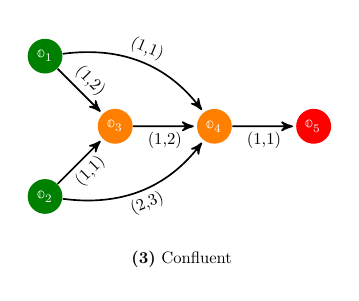
\begin{tikzpicture}[->,>=stealth',shorten >=1pt,auto,node distance=2.1cm,
                    semithick,scale=0.6, every node/.style={scale=0.6}]
    \node[shape=circle,fill=black!50!green,draw=none,text=white] (A)                    {$\mathbb{o}_1$};
  \node[shape=circle,fill=orange,draw=none,text=white] (D) [below right of=A] {$\mathbb{o}_3$};
        \node[shape=circle,fill=black!50!green,draw=none,text=white] (C) [below left of=D] {$\mathbb{o}_2$};

  \node[shape=circle,fill=orange,draw=none,text=white] (E) [right of=D]       {$\mathbb{o}_4$};
  \node[shape=circle,fill=red,draw=none,text=white] (F) [right of=E]       {$\mathbb{o}_5$};
  \node[anchor=west] at (1.7,-4.3) (X) {\textbf{(3)} Confluent};
  \path (A) edge    node [sloped, above] {(1,2)}           (D)
  edge [bend left] node [sloped, above] {(1,1)} (E)
        (C) edge    node [sloped, below]{(1,1)}          (D)
            edge  [bend right]   node [sloped, below] {(2,3)}  (E)
        (E) edge node [sloped, below] {(1,1)} (F)
        (D) edge    node [sloped, below] {(1,2)} (E);
\end{tikzpicture}
\end{center}
\begin{center}
  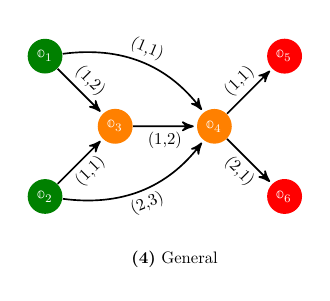
\begin{tikzpicture}[->,>=stealth',shorten >=1pt,auto,node distance=2.1cm,
                    semithick,scale=0.6, every node/.style={scale=0.6}]
    \node[shape=circle,fill=black!50!green,draw=none,text=white] (A)                    {$\mathbb{o}_1$};
  \node[shape=circle,fill=orange,draw=none,text=white] (D) [below right of=A] {$\mathbb{o}_3$};
        \node[shape=circle,fill=black!50!green,draw=none,text=white] (C) [below left of=D] {$\mathbb{o}_2$};

  \node[shape=circle,fill=orange,draw=none,text=white] (E) [right of=D]       {$\mathbb{o}_4$};
    \node[shape=circle,fill=red,draw=none,text=white] (G) [below right of=E]       {$\mathbb{o}_6$};
  \node[shape=circle,fill=red,draw=none,text=white] (F) [above right of=E]       {$\mathbb{o}_5$};
  \node[anchor=west] at (1.7,-4.3) (X) {\textbf{(4)} General};
  \path (A) edge    node [sloped, above]  {(1,2)}          (D)
  edge [bend left] node [sloped, above] {(1,1)} (E)
        (C) edge    node [sloped, below]{(1,1)}          (D)
            edge  [bend right]   node [sloped, below] {(2,3)}  (E)
        (E) edge node [sloped, above] {(1,1)} (F)
            edge node [sloped, below] {(2,1)} (G)
        (D) edge    node [sloped, below] {(1,2)} (E);
\end{tikzpicture}
\end{center}
\end{multicols}


\only<1>{\begin{block}{Definition \textbf{Enrichment Graph}}
\begin{center}
Let $G=(\mathbf{V},\mathbf{E},\mathbf{L},\Phi,\Psi)$ be a directed acyclic labeled multigraph.  
\end{center}
\begin{multicols}{3}
\noindent\begin{equation*}
\begin{aligned}
  \mathbf{L}\colon E & \to 2^{(\mathbb{N} \times \mathbb{N})} \\
  e = (u,v) & \mapsto \left\{ (i_1, j_1), \dots, (i_n, j_n) \right\}
\end{aligned}
\label{eq:labelf}
\end{equation*}\noindent
\begin{equation*}
\begin{aligned}
  \Phi \colon \mathbf{V} & \to \mathbb{O} \\
  v & \mapsto \mathbb{o}_{(n,m)}
\end{aligned}
\label{eq:labelf}
\end{equation*}\noindent
\begin{equation*}
\begin{aligned}
  \Psi \colon \mathbf{V} & \to \mathcal{D} \\
  v & \mapsto P
\end{aligned}
\label{eq:labelf}
\end{equation*}
\end{multicols}
\break
\end{block}}
\end{frame}

\subsection{An Efficient Representation}
\begin{frame}{Enrichment Tables - An Efficient Representation for Learning}
\begin{figure}[tb]
\centering
  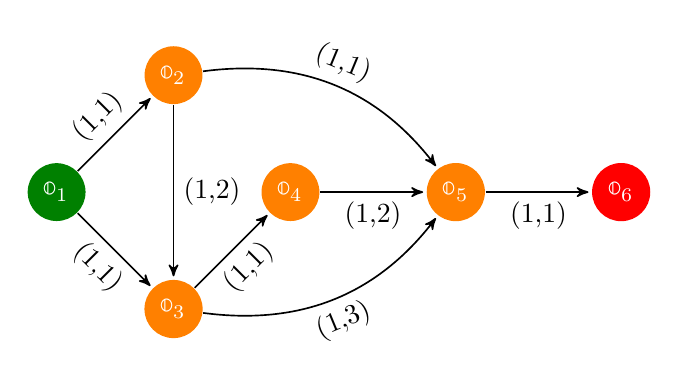
\begin{tikzpicture}[->,>=stealth',shorten >=1pt,auto,node distance=2.1cm,
                    semithick]

  \node[shape=circle,fill=black!50!green,draw=none,text=white] (B)  {$\mathbb{o}_1$};
    \node[shape=circle,fill=orange,draw=none,text=white] (A) [above right of=B]                   {$\mathbb{o}_2$};
      \node[shape=circle,fill=orange,draw=none,text=white] (C) [below right of=B] {$\mathbb{o}_3$};
  \node[shape=circle,fill=orange,draw=none,text=white] (D) [below right of=A] {$\mathbb{o}_4$};

  \node[shape=circle,fill=orange,draw=none,text=white] (E) [right of=D]       {$\mathbb{o}_5$};
  \node[shape=circle,fill=red,draw=none,text=white] (F) [right of=E]       {$\mathbb{o}_6$};

  \path (A) edge    node  {(1,2)}           (C)
  edge [bend left] node [sloped, above] {(1,1)} (E)
        (B) edge    node [sloped, below]{(1,1)}          (C)
            edge    node [sloped, above]{(1,1)}          (A)
        (C) edge    node [sloped, below]{(1,1)}          (D)
            edge  [bend right]   node [sloped, below] {(1,3)}  (E)
        (E) edge node [sloped, below] {(1,1)} (F)
        (D) edge    node [sloped, below] {(1,2)} (E);
\end{tikzpicture}
\end{figure}
  \begin{table}[tb]
\centering
\begin{tabular}{lc|c|c|c|c|c}
  \rowcolor{black!50!green}
  1: & $\mathbb{o}_1$ & $P_1$ & 0 & 0 & 0 & 0\\ \hline
  \rowcolor{orange}
  2: & $\mathbb{o}_2$ & $P_2$ & 1 & 1 & 0 & 0\\ \hline
  \rowcolor{orange}
  3: & $\mathbb{o}_3$ & $P_3$ & 2 & 1 & 2 & 0\\ \hline
  \rowcolor{orange}
  4: & $\mathbb{o}_4$ & $P_4$ & 1 & 3 & 0 & 0\\ \hline
  \rowcolor{darkred!70}
  5: & $\mathbb{o}_5$ & $P_5$ & 3 & 2 & 4 & 3
\end{tabular}
\end{table}
\end{frame}

\subsection{Baseline GP Algorithm}


\begin{frame}{Learning Problem}
\begin{itemize}[<+->]
  \item Restrict leaning problem to
  \begin{itemize}
    \item   \textbf{inherently confluent enrichment graphs}
     \item   enrichment operators with in-degree in $\{1,2\}$
     \item regularly shaped RDF datasets
  \end{itemize}    
  \item Training data
  \begin{itemize}
    \item source training datasets(s) ($\leq 2$)
     \item  and target training dataset ($=1$)
  \end{itemize}
  \item Learn enrichment table using Genetic Programming (GP) and Multi-Expression Programming (MEP)
  \item Use linear combination of $F_1$ measure on subjects, predicates, objects and whole triples as fitness function
\end{itemize}
\end{frame}



\begin{frame}{Genetic Programming Algorithm}
  \begin{itemize}[<+->]
    \item ($\mu + \lambda$) Genetic Algorithm:
    \item Initialize current population $p_c$
    \item Repeat until termination criterion is met:
      \begin{itemize}
        \item Evaluate the current population $p_c$
        \item Initialize the next population with elite $p_n\coloneq \left\{\text{best}(p_c)\right\}$
        \item Fill the mating pool $p_m$ with $\mu$ individuals using tournament selection on $p_c$
        \item Apply crossover randomly to pairs $(\mathbb{T}_1,\mathbb{T}_2)\in p_m$
        \item Insert resulting childs into $p_n$
        \item Insert $\lambda - \mu$ individuals into $p_n$ using tournament selection on $p_c$
        \item Apply mutation to each individual $\mathbb{T}\in p_n$ with probability $\sigma$
        \item For each row $\mathbb{T}_i$ of individuals chosen for mutation, mutate the row with probability $\rho$
      \end{itemize}
  \end{itemize}
\end{frame}


\begin{frame}{Multi-Expressive Enrichment Tables}
\begin{itemize}[<+->]
  \item MEP: One genotype represents multiple solutions (phenotypes)
  \item Use MEP for enrichment tables
  \item Called multi-expressive enrichment table
\end{itemize}
  \begin{center}
\begin{tabular}{lc|c|c|c|c|c}
  \rowcolor{green!50!black}
  1: & $\mathbb{o}_1$ & $P_1$ & 0 & 0 & 0 & 0\\ \hline
  \rowcolor{orange}
  2: & $\mathbb{o}_2$ & $P_2$ & 1 & 1 & 0 & 0\\ \hline
  \rowcolor{orange}
  3: & $\mathbb{o}_3$ & $P_3$ & 2 & 1 & 2 & 0\\ \hline
  \rowcolor{orange}
  4: & $\mathbb{o}_6$ & $P_6$ & 2 & 3 & 1 & 0\\ \hline
  \rowcolor{orange}
  5: & $\mathbb{o}_4$ & $P_4$ & 1 & 3 & 0 & 0\\ \hline
  \rowcolor{darkred!70}
  6: & $\mathbb{o}_7$ & $P_7$ & 1 & 5 & 0 & 0\\ \hline
  \rowcolor{orange}
  7: & $\mathbb{o}_8$ & $P_8$ & 2 & 4 & 3 & 0\\ \hline
  \rowcolor{darkred!70}
  8: & $\mathbb{o}_5$ & $P_5$ & 3 & 2 & 5 & 3\\ \hline
  \rowcolor{darkred!70}
  9: & $\mathbb{o}_9$ & $P_9$ & 1 & 7 & 0 & 0
\end{tabular} 
\end{center}
\end{frame}

\begin{frame}[fragile]{Population Initialization}
\begin{multicols}{2}
{\only<1>{
\begin{itemize}
  \item Add all dataset emitters
\end{itemize}
}\only<2-3>{
\begin{itemize}
  \item Add all dataset emitters
  \item Randomly generate rows
\end{itemize}
}}
  \begin{center}
{\only<1>{
\begin{tabular}{lc|c|c|c|c|c}
  \rowcolor{green!50!black}
  1: & $\mathbb{o}_1$ & $P_1$ & 0 & 0 & 0 & 0\\ \hline
\end{tabular}}
\only<2>{
\begin{tabular}{lc|c|c|c|c|c}
  \rowcolor{green!50!black}
  1: & $\mathbb{o}_1$ & $P_1$ & 0 & 0 & 0 & 0\\ \hline
  \rowcolor{orange}
  2: & $\mathbb{o}_2$ & $\emptyset$ & 1 & 1 & 0 & 0\\ \hline
\end{tabular}}
\only<3>{
\begin{tabular}{lc|c|c|c|c|c}
  \rowcolor{green!50!black}
  1: & $\mathbb{o}_1$ & $P_1$ & 0 & 0 & 0 & 0\\ \hline
  \rowcolor{orange}
  2: & $\mathbb{o}_2$ & $\emptyset$ & 1 & 1 & 0 & 0\\ \hline
  \rowcolor{orange}
  3: & $\mathbb{o}_3$ & $\emptyset$ & 2 & 1 & 2 & 0\\ \hline
  \rowcolor{orange}
  4: & $\mathbb{o}_6$ & $\emptyset$ & 2 & 3 & 1 & 0\\ \hline
  \rowcolor{orange}
  5: & $\mathbb{o}_4$ & $\emptyset$ & 1 & 3 & 0 & 0\\ \hline
  \rowcolor{darkred!70}
  6: & $\mathbb{o}_7$ & $\emptyset$ & 1 & 5 & 0 & 0\\ \hline
  \rowcolor{orange}
  7: & $\mathbb{o}_8$ & $\emptyset$ & 2 & 4 & 3 & 0\\ \hline
  \rowcolor{darkred!70}
  8: & $\mathbb{o}_5$ & $\emptyset$ & 3 & 2 & 5 & 3\\ \hline
  \rowcolor{darkred!70}
  9: & $\mathbb{o}_9$ & $\emptyset$ & 1 & 7 & 0 & 0
\end{tabular}}}
\end{center}
\end{multicols}
\end{frame}

\subsection{Enrichment Table Compaction}

\begin{frame}{Enrichment Table Compaction}

\begin{multicols}{2}
\begin{center}
\begin{tabular}{lc|c|c|c|c|c}
  \rowcolor{green!50!black}
  1: & $\mathbb{o}_1$ & $P_1$ & 0 & 0 & 0 & 0\\ \hline
  \rowcolor{orange}
  2: & $\mathbb{o}_2$ & $P_2$ & 1 & 1 & 0 & 0\\ \hline
  \rowcolor{orange}
  3: & $\mathbb{o}_3$ & $P_3$ & 2 & 1 & 2 & 0\\ \hline
  \rowcolor{orange}
  4: & $\mathbb{o}_6$ & $P_6$ & 2 & 3 & 1 & 0\\ \hline
  \rowcolor{orange}
  5: & $\mathbb{o}_4$ & $P_4$ & 1 & 3 & 0 & 0\\ \hline
  \rowcolor{darkred!70}
  6: & $\mathbb{o}_7$ & $P_7$ & 1 & 5 & 0 & 0\\ \hline
  \rowcolor{orange}
  7: & $\mathbb{o}_8$ & $P_8$ & 2 & 4 & 3 & 0\\ \hline
  \rowcolor{darkred!70}
  8: & $\mathbb{o}_5$ & $P_5$ & 3 & 2 & 5 & 3\\ \hline
  \rowcolor{darkred!70}
  9: & $\mathbb{o}_9$ & $P_9$ & 1 & 7 & 0 & 0
\end{tabular} 
\end{center}
\begin{center}
\begin{tabular}{lc|c|c|c|c|c}
  \rowcolor{green!50!black}
  1: & $\mathbb{o}_1$ & $P_1$ & 0 & 0 & 0 & 0\\ \hline
  \rowcolor{orange}
  2: & $\mathbb{o}_2$ & $P_2$ & 1 & 1 & 0 & 0\\ \hline
  \rowcolor{orange}
  3: & $\mathbb{o}_3$ & $P_3$ & 2 & 1 & 2 & 0\\ \hline
  \rowcolor{black!60}
  4: & $\mathbb{o}_6$ & $P_6$ & 2 & 3 & 1 & 0\\ \hline
  \rowcolor{orange}
  5: & $\mathbb{o}_4$ & $P_4$ & 1 & 3 & 0 & 0\\ \hline
  \rowcolor{black!60}
  6: & $\mathbb{o}_7$ & $P_7$ & 1 & 5 & 0 & 0\\ \hline
  \rowcolor{black!60}
  7: & $\mathbb{o}_8$ & $P_8$ & 2 & 4 & 3 & 0\\  \hline
  \rowcolor{darkred!70}
  8: & $\mathbb{o}_5$ & $P_5$ & 3 & 2 & 5 & 3\\ \hline
  \rowcolor{black!60}
  9: & $\mathbb{o}_9$ & $P_9$ & 1 & 7 & 0 & 0 
\end{tabular}  
\end{center}
\end{multicols}
\begin{textblock*}{3cm}(7.4cm, -2.4cm) % {block width} (coords)
$\to$
\end{textblock*}
\end{frame}

\begin{frame}{Enrichment Table Compaction II}

\begin{multicols}{2}
\begin{center}
\begin{tabular}{lc|c|c|c|c|c}
  \rowcolor{green!50!black}
  1: & $\mathbb{o}_1$ & $P_1$ & 0 & 0 & 0 & 0\\ \hline
  \rowcolor{orange}
  2: & $\mathbb{o}_2$ & $P_2$ & 1 & 1 & 0 & 0\\ \hline
  \rowcolor{orange}
  3: & $\mathbb{o}_3$ & $P_3$ & 2 & 1 & 2 & 0\\ \hline
  \rowcolor{black!60}
  4: & $\mathbb{o}_6$ & $P_6$ & 2 & 3 & 1 & 0\\ \hline
  \rowcolor{orange}
  5: & $\mathbb{o}_4$ & $P_4$ & 1 & 3 & 0 & 0\\ \hline
  \rowcolor{black!60}
  6: & $\mathbb{o}_7$ & $P_7$ & 1 & 5 & 0 & 0\\ \hline
  \rowcolor{black!60}
  7: & $\mathbb{o}_8$ & $P_8$ & 2 & 5 & 3 & 0\\  \hline
  \rowcolor{darkred!70}
  8: & $\mathbb{o}_5$ & $P_5$ & 3 & 2 & 5 & 3\\ \hline
  \rowcolor{black!60}
  9: & $\mathbb{o}_9$ & $P_9$ & 1 & 7 & 0 & 0 
\end{tabular} 
\end{center}
\begin{center}
\begin{tabular}{lc|c|c|c|c|c}
  \rowcolor{green!50!black}
  1: & $\mathbb{o}_1$ & $P_1$ & 0 & 0 & 0 & 0\\ \hline
  \rowcolor{orange}
  2: & $\mathbb{o}_2$ & $P_2$ & 1 & 1 & 0 & 0\\ \hline
  \rowcolor{orange}
  3: & $\mathbb{o}_3$ & $P_3$ & 2 & 1 & 2 & 0\\ \hline
  \rowcolor{orange}
  \color{green}{\textbf{4}}: & $\mathbb{o}_4$ & $P_4$ & 1 & 3 & 0 & 0\\ \hline
  \rowcolor{darkred!70}
  \color{green}{\textbf{5}}: & $\mathbb{o}_5$ & $P_5$ & 3 & 2 & \color{green}{\textbf{4}} & 3\\ \hline
\end{tabular}  
\end{center}
\end{multicols}
\begin{textblock*}{3cm}(7.4cm, -3.4cm) % {block width} (coords)
$\to$
\end{textblock*}
\end{frame}

\subsection{Semantic Genetic Operators}

\begin{frame}{Semantic Genetic Operators}
  \begin{itemize}[<+->]
    \item Take into account the problem domain
    \item More like a guided search, not completely random
    \item Intereseting properties of our problem domain:
    \begin{itemize}
      \item Structure of the graph
      \item Applicability of enrichment operators
    \end{itemize}

  \end{itemize}
\end{frame}


\begin{frame}{Graph Merging Crossover}
  \begin{itemize}[<+->]
    \item Idea: select two most promising phenotypes
    \item $\to$ combine them into a new genotype
    \item With probability of $0.25$: insert an enrichment operator merging both together
  \end{itemize}
\end{frame}


\begin{frame}{Pre- \& Postcondition Mutation}
  \begin{itemize}[<+->]
    \item Idea: method on enrichment operators states applicability
    \item Select row for mutation
    \item Broadcast pre-/postconditions to operators
    \item Operators return applicability
    \item Roulette wheel selection proportionate on applicability
  \end{itemize}
\end{frame}

\section{Evaluation}
\begin{frame}{Evaluation Setup}
\begin{itemize}
  \item \textbf{Fist set of experiments:} Hyperparameter Optimization
  \begin{itemize}
  \item Grid search
  \item Mutation probability $\sigma \in \{0.1,0.3,0.5,0.7,0.9\}$
  \item Mutation rate $\rho \in \{0.1,0.3,0.5,0.7,0.9\}$
  \item Offspring fraction $\alpha = \frac{\lambda}{\mu} \in \{0, 0.2, 0.4, 0.6, 0.8, 1.0 \} $
  \end{itemize}
  \item \textbf{Second set of experiments:} Performance on real world example
\end{itemize}
\end{frame}

\subsection{Hyperparameter Optimization}
\begin{frame}{Hyperparameter Optimization}
\begin{itemize}
  \item Very simple toy learning problem
  \item 3 enrichment operators, order does not matter
  \item only baseline algorithm ($\mu = 30, r=7, g=5000$)
  \item 1000 repetitions
  \item best set of parameter $(\alpha/\sigma/\rho)=(1.0/0.9/0.9)$
\end{itemize}
\begin{center}
  \includegraphics[page=1]{gfx/graphs}
\end{center}
\end{frame}

\begin{frame}{Hyperparameter Optimization}
\begin{itemize}
  \item Very simple toy learning problem
  \item 3 enrichment operators, order does not matter
  \item with enrichment table compaction enabled
  \item 1000 repetitions
  \item best set of parameter $(\alpha/\sigma/\rho)=(0.0/0.1/0.1)$
\end{itemize}
\begin{center}
  \includegraphics[page=2]{gfx/graphs}
\end{center}
\end{frame}

\begin{frame}{Hyperparameter Optimization}
\begin{itemize}
  \item Much harder problem
  \item 5 enrichment operators, order \emph{does matter}
  \item with all optimizations enabled
  \item 1000 repetitions
  \item best set of parameter $(\alpha/\sigma/\rho)=(1.0/0.5/0.5)$
\end{itemize}
\begin{center}
  \includegraphics[page=3]{gfx/graphs}
\end{center}
\end{frame}


\subsection{Performance on Real World Example}
\begin{frame}{Performance on Real World Example}
\begin{center}
  \includegraphics[page=1, width=0.8\textwidth]{gfx/img}
\end{center}
\end{frame}


\begin{frame}{Performance on Real World Example}
\begin{center}
    \includegraphics[page=2, width=\textwidth]{gfx/img}
\end{center}
\end{frame}


\begin{frame}{Performance on Real World Example}
\begin{multicols}{2}
  \begin{center}
    \includegraphics[page=4, width=0.4\textwidth]{gfx/graphs}
\end{center}  
\begin{itemize}[<+->]
  \item 50 repetitions
  \item maximum 2000 generations
  \item $\mu=30, \alpha=1, \sigma=0.5, \rho=0.5$
  \item measure best fitness in each generation
  \item compute average fitness for each generation
  \item compute $95\%$-confidence intervals using Students $t$-distribution
  \item Result: on average solution quality over $99\%$ after $500$ generations with $95\%$-confidence interval of $\pm 0.6\%$
\end{itemize}
\end{multicols}
\end{frame}

\section{Conclusion}

\begin{frame}
\begin{itemize}[<+->]
  \item Implemented a tool for generalistic DAG-shaped enrichment workflows
  \item Developed a classification of enrichment graphs
  \item Derived a GP- and MEP-based learning approach for inherently confluent enrichment graphs
  \item Supplied several optimizations
  \item Optimizations successfully improved solution quality \& time to convergence
  \item Over $99\%$ after $500$ generations with $95\%$-confidence interval of $\pm 0.6\%$ in a real-world test case
\end{itemize}  
\end{frame}

\begin{frame}{Thank You for Your Attention}

\end{frame}



\end{document}
